% Phase-II Report -- EcoGraph: Graph Based Algorithmic Waste Management
% Built on the department-supplied Phase-2.tex progress template.
% Compile with pdfLaTeX. geulogo.png and the member photos (tejas.jpeg, apoorv.jpeg, yash.jpeg) sit in this folder.

\documentclass[12pt,a4paper]{article}

% ============================================================
% PACKAGES
% ============================================================
\usepackage[
    a4paper,
    top=1.55cm,
    bottom=1.35cm,
    left=1.75cm,
    right=1.75cm
]{geometry}

\usepackage[T1]{fontenc}
\usepackage{newtxtext}
\usepackage{graphicx}
\usepackage{xcolor}
\usepackage{array}
\usepackage{tabularx}
\usepackage{fancyhdr}
\usepackage{tikz}
\usepackage{eso-pic}
\usepackage{ragged2e}
\usepackage{enumitem}
\usepackage{amsmath}
\usepackage[hidelinks]{hyperref}
\usetikzlibrary{positioning,arrows.meta,decorations.pathreplacing,calc}

\definecolor{DiagFill}{RGB}{238,244,251}
\definecolor{DiagGrey}{RGB}{90,90,90}

% plain-language formula block: \formula{line \\ line}
\newcommand{\formula}[1]{%
    \begin{center}
    \colorbox{DiagFill}{\parbox{0.92\linewidth}{\vspace{4pt}\centering\fontsize{10}{14}\selectfont #1\vspace{4pt}}}
    \end{center}
}

% boxed figure that continues the Approach section: \diagbox{title}{body}
\newcommand{\diagbox}[2]{%
    \par\noindent
    \fbox{\begin{minipage}{\dimexpr\textwidth-2\fboxsep-2\fboxrule\relax}
        \vspace{4pt}
        {\color{GEUBlue}\bfseries\fontsize{11.5}{14}\selectfont #1}
        \vspace{4pt}

        \fontsize{10}{12.5}\selectfont
        #2
        \vspace{4pt}
    \end{minipage}}\par
}

% ============================================================
% COLORS
% ============================================================
\definecolor{GEUBlue}{RGB}{43,91,145}
\definecolor{GEUBannerBlue}{RGB}{0,102,148}
\definecolor{GEUYellow}{RGB}{255,201,38}
\definecolor{InstructionGrey}{RGB}{125,125,125}

% ============================================================
% GENERAL SETTINGS
% ============================================================
\setlength{\parindent}{0pt}
\setlength{\parskip}{0pt}
\renewcommand{\arraystretch}{1}
\setlist{leftmargin=5mm,itemsep=1pt,topsep=2pt,parsep=0pt}

% ============================================================
% HEADER / FOOTER
% ============================================================
\pagestyle{fancy}
\fancyhf{}

\fancyhead[L]{%
    \fontsize{10.5}{12}\selectfont
    DSA \& OOPs in C++ -- Team DSCPP-III-2026-T186
}

\fancyhead[R]{%
    \fontsize{10.5}{12}\selectfont
    PHASE-II PROJECT PROGRESS
}

\fancyfoot[R]{%
    \fontsize{10}{12}\selectfont
    Page \thepage
}

\renewcommand{\headrulewidth}{0pt}
\renewcommand{\footrulewidth}{0pt}

\setlength{\headheight}{20pt}
\setlength{\headsep}{0.65cm}
\setlength{\footskip}{0.65cm}

% ============================================================
% BOTTOM YELLOW LINE
% ============================================================
\AddToShipoutPictureBG{%
\begin{tikzpicture}[remember picture,overlay]
    \fill[GEUYellow]
    (current page.south west)
    rectangle
    ([yshift=0.14cm]current page.south east);
\end{tikzpicture}
}

% ============================================================
% CUSTOM COMMANDS
% ============================================================
\newcommand{\sectiontitle}[1]{%
    {\color{GEUBlue}
    \fontsize{18}{22}\selectfont #1}
}

\newcommand{\instruction}[1]{%
    {\color{InstructionGrey}
    \fontsize{10.5}{13}\selectfont #1}
}

\newcommand{\answerbox}[2]{%
    \begin{tabularx}{\textwidth}{
        |>{\raggedright\arraybackslash}X|}
        \hline
        \parbox[t][#1][t]{\dimexpr\linewidth-12pt\relax}{
            \vspace{5pt}
            \fontsize{11}{13.5}\selectfont
            \setlength{\parskip}{4pt}
            #2
        }\\
        \hline
    \end{tabularx}
}

% one row of the two-column task tables
\newcommand{\taskrow}[2]{%
    \parbox[t]{\linewidth}{\vspace{3pt}\fontsize{10.5}{12.5}\selectfont #1\vspace{4pt}}
    &
    \parbox[t]{\linewidth}{\vspace{3pt}\fontsize{10.5}{12.5}\selectfont #2\vspace{4pt}}
    \\
    \hline
}

% ============================================================
% DOCUMENT
% ============================================================
\begin{document}

% ============================================================
% PAGE 1
% ============================================================

\vspace*{0.10cm}


\includegraphics[width=8.0cm]{geulogo.png}

\vspace{0.70cm}

\noindent
\colorbox{GEUBannerBlue}{%
\parbox{\dimexpr\textwidth-2\fboxsep\relax}{
    \vspace{0.17cm}
    {\color{GEUYellow}
    \fontsize{16.5}{20}\selectfont
    \bfseries
    PROJECT AND TEAM INFORMATION}
    \vspace{0.17cm}
}}

\vspace{0.80cm}

% PROJECT TITLE
\sectiontitle{Project Title}

\vspace{0.05cm}

\instruction{(Try to choose a catchy title. Max 20 words).}

\vspace{0.40cm}

\answerbox{1.45cm}{EcoGraph: Graph-Based Algorithmic Waste Management with Hazard-Aware Routing and Fill-Rate-Adaptive Collection Scheduling}

\newpage

% STUDENT / TEAM INFORMATION
\vspace*{0.15cm}

\sectiontitle{Student/Team Information}

\vspace{0.40cm}

\noindent
\begin{tabularx}{\textwidth}{|>{\RaggedRight\arraybackslash}p{0.69\textwidth}|>{\RaggedRight\arraybackslash}X|}
\hline
\begin{minipage}[t]{\linewidth}
\vspace{1.5mm}
\textit{Team Name:}\\[-1mm]
\textit{Team \#}\\[-1mm]
\textit{PBL Mentor:}
\vspace{1.5mm}
\end{minipage}
&
\begin{minipage}[t]{\linewidth}
\vspace{1.5mm}
\textit{EcoGraph}\\[-1mm]
\textit{DSCPP-III-2026-T186}\\[-1mm]
\textit{Mr. Navneet Rajput}
\vspace{1.5mm}
\end{minipage}
\\
\hline
\begin{minipage}[t][6.0cm][t]{\linewidth}
\vspace{1.5mm}
\textbf{Team member 1 (Team Lead)}\\[-1mm]
\textit{(Last Name, name: student ID: email, picture):}
\vspace{2.0cm}
\end{minipage}
&
\begin{minipage}[t][6.0cm][t]{\linewidth}
\vspace{1.5mm}
\textit{Jain, Tejas}\\
\textit{Student ID: 2510011541}\\
\textit{Roll No. 2028228, Sec A}\\
\textit{aispace101@gmail.com}

\vspace{1.5mm}
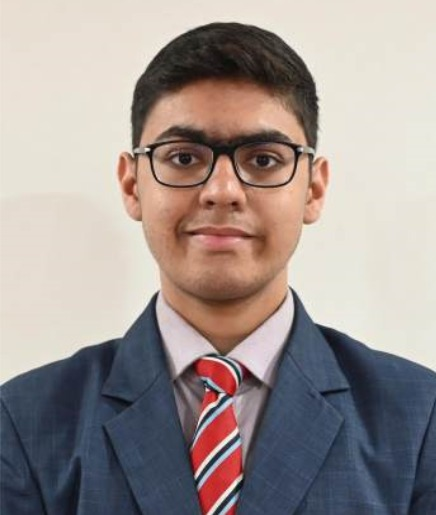
\includegraphics[width=3.0cm,height=3.2cm,keepaspectratio]{tejas.jpeg}
\end{minipage}
\\
\hline
\begin{minipage}[t][6.0cm][t]{\linewidth}
\vspace{1.5mm}
\textbf{Team member 2}\\[-1mm]
\textit{(Last Name, name: student ID: email, picture):}
\vspace{2.0cm}
\end{minipage}
&
\begin{minipage}[t][6.0cm][t]{\linewidth}
\vspace{1.5mm}
\textit{Negi, Apoorv}\\
\textit{Student ID: 2510011088}\\
\textit{Roll No. 2027640, Sec D}\\
\textit{apoorvnegi17@gmail.com}

\vspace{1.5mm}
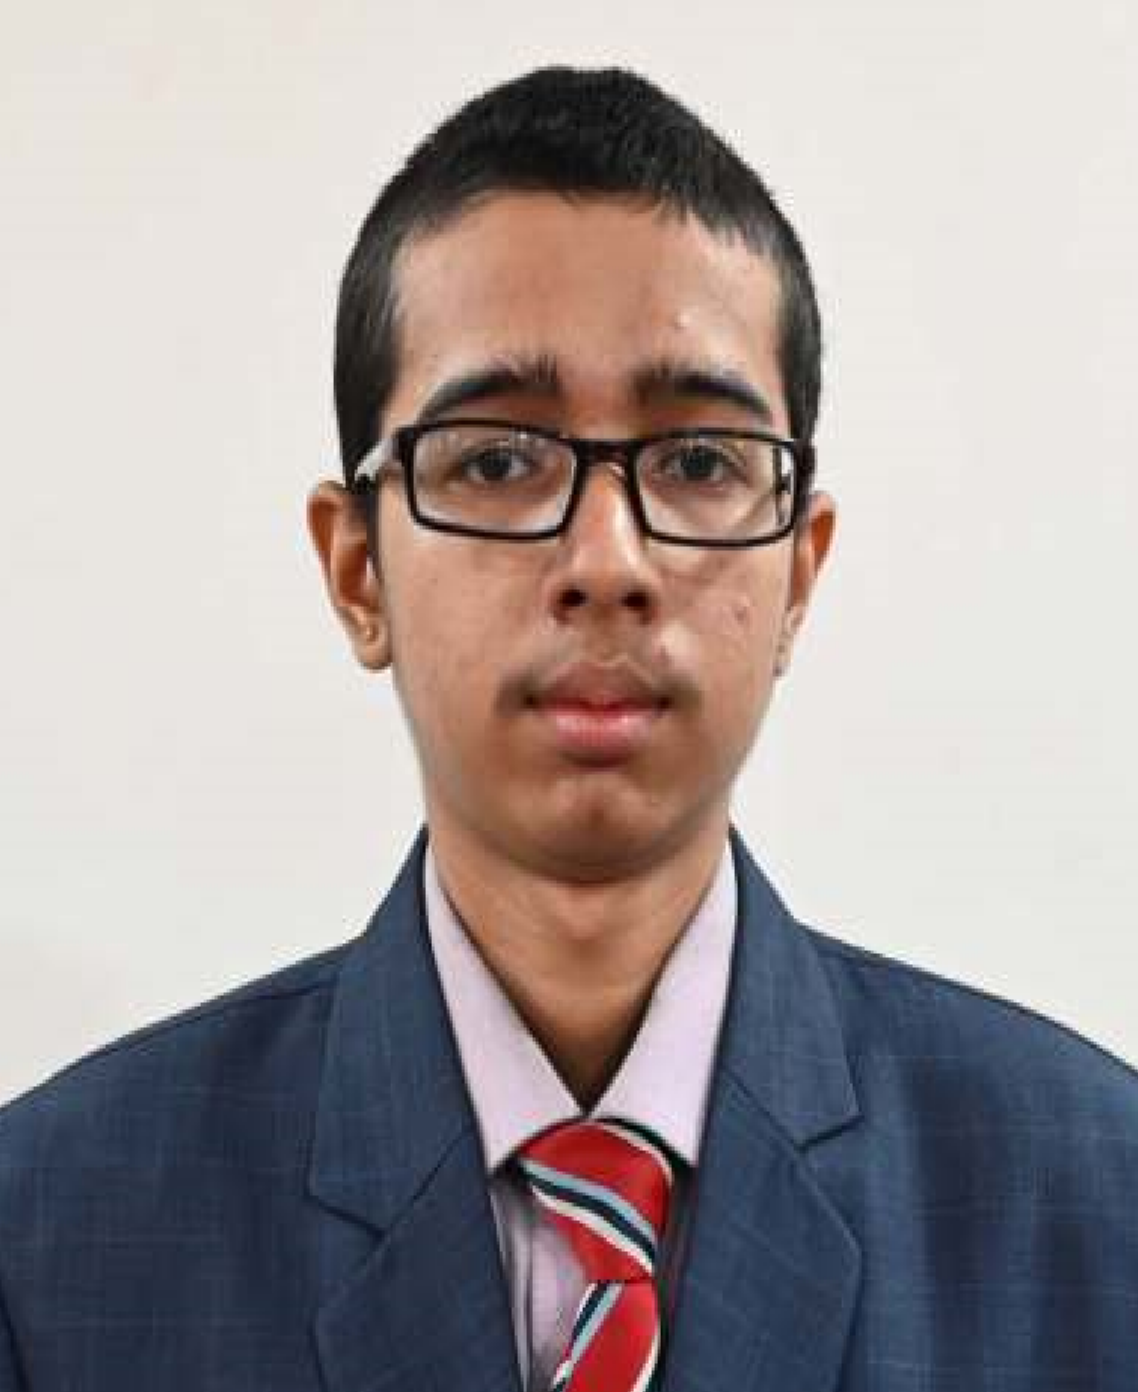
\includegraphics[width=3.0cm,height=3.2cm,keepaspectratio]{apoorv.jpeg}
\end{minipage}
\\
\hline
\begin{minipage}[t][6.0cm][t]{\linewidth}
\vspace{1.5mm}
\textbf{Team member 3}\\[-1mm]
\textit{(Last Name, name: student ID: email, picture):}
\vspace{2.0cm}
\end{minipage}
&
\begin{minipage}[t][6.0cm][t]{\linewidth}
\vspace{1.5mm}
\textit{Nigam, Yash}\\
\textit{Student ID: 2510010441}\\
\textit{Roll No. 2028289, Sec H}\\
\textit{nigamyash07@gmail.com}

\vspace{1.5mm}
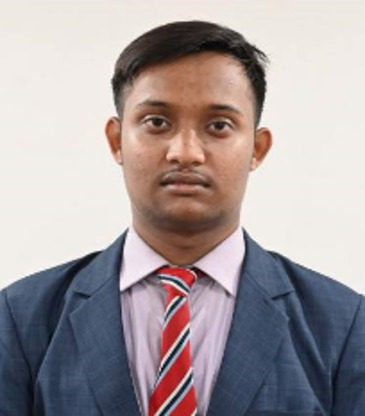
\includegraphics[width=3.0cm,height=3.2cm,keepaspectratio]{yash.jpeg}
\end{minipage}
\\
\hline
\end{tabularx}

\newpage
% ============================================================
% PAGE 2
% ============================================================

\vspace*{0.15cm}

\noindent
\colorbox{GEUBannerBlue}{%
\parbox{\dimexpr\textwidth-2\fboxsep\relax}{
    \vspace{0.18cm}
    {\color{GEUYellow}
    \fontsize{17}{21}\selectfont
    \bfseries
    PHASE-II PROJECT PROGRESS DESCRIPTION (35 pts)}
    \vspace{0.18cm}
}}

\vspace{0.70cm}

% PROJECT ABSTRACT
\sectiontitle{Project Abstract (2 pts)}

\vspace{0.05cm}

\instruction{
(Brief restatement of your project's main goal. Max 300 words).
}

\vspace{0.12cm}

\answerbox{6.55cm}{Garbage trucks in most Indian cities still run the same fixed route every day, whether a street has anything to collect or not. Bins that fill fast overflow, bins that barely fill get visited anyway, and hazardous waste like used syringes or old batteries is often picked up by the same truck, on the same roads, as kitchen scraps.

EcoGraph is our attempt to fix that with plain graph algorithms. We model Dehradun as a weighted graph of depots, homes, road junctions and disposal bins, where every road carries a distance in km and a zone tag: residential, commercial, industrial or arterial. On top of that graph the system does three jobs. It works out which homes and bins are actually due for pickup from how fast each one fills. It builds a shortest-path collection route for each truck using Dijkstra's algorithm. And whenever a waste description reads as medical or chemical, it sends a separate truck that is only allowed on industrial and arterial roads, so that waste never passes through a neighbourhood or a market.

Everything runs inside one C++17 server that also serves a browser front end, where you can watch trucks move across the map and step the city forward day by day to see how the schedule holds up.}

\newpage

% UPDATED PROJECT APPROACH
\sectiontitle{Updated Project Approach and Architecture (2 pts)}

\vspace{0.05cm}

\instruction{
(Describe your current approach, including system design,
communication protocols, libraries used, etc.\\
Max 300 words).
}

\vspace{0.25cm}

\answerbox{14.7cm}{\textbf{Design.} One C++17 process serves the REST API and the front end on one port. \texttt{controllers.cpp} handles HTTP and JSON behind a mutex; domain classes (\texttt{Graph}, Dijkstra, \texttt{Scheduler}, classifier, route builders, \texttt{Simulation}) work on an in-memory adjacency-list city loaded from \texttt{city.json}.

\textbf{Routing.} \texttt{RouteStrategy} is an abstract base class; the Priority and FIFO subclasses set the stop order.

\textbf{Protocol.} REST over HTTP with JSON, 13 endpoints, one error format.

\textbf{Front end.} Plain JavaScript with no build step, plus a day-by-day simulation, a limited fleet and a city builder.

\textbf{Libraries.} cpp-httplib, nlohmann/json, Cytoscape.js.

\vspace{2mm}
{\color{GEUBlue}\bfseries\fontsize{12}{14}\selectfont One day, step by step} \quad {\small(diagrams (a)--(g) below)}

\textbf{1.} The clock moves forward one day.

\textbf{2.} A home is due once the days since its last collection reach capacity / fill rate (1--14 days); the most overdue comes first (c).

\textbf{3.} Due bins are emptied, hazardous homes go to the hazard trucks (f), and normal homes are ordered and packed onto trucks before routing (e).

\textbf{4.} Each truck chains shortest paths in its list order:
\formula{\raggedright\ttfamily\small
current = DEPOT;\ \ visited = \{ \}\\
for each home in order:\\
\hspace*{4mm}skip it if in visited\\
\hspace*{4mm}path = Dijkstra(current $\to$ home);\ \ if none, mark unreachable\\
\hspace*{4mm}empty later stops on the path, add them to visited\hfill\textrm{\small(en-route pickup, (d))}\\
\hspace*{4mm}empty home, add to visited;\ \ current = home\\
then visit the nearest bin for each waste type collected}

\textbf{5.} Served homes get ``last collected = today''; unreachable ones are reported as failed, and carried-over homes rank higher tomorrow.}

\vspace{0.35cm}

% ------------------------------------------------------------
% APPROACH: DIAGRAMS
% ------------------------------------------------------------

\diagbox{(a) System Pipeline}{%
\begin{center}
\begin{tikzpicture}[
node distance=8mm,
box/.style={rectangle,rounded corners,draw=GEUBlue,fill=DiagFill,thick,minimum width=2.4cm,minimum height=12mm,align=center,font=\scriptsize\sffamily},
arrow/.style={-{Latex[length=2mm]},thick,draw=GEUBlue}
]
\node[box] (a) {Browser UI\\JS + Cytoscape.js};
\node[box,right=of a] (b) {HTTP layer\\cpp-httplib};
\node[box,right=of b] (c) {Controllers\\JSON + mutex};
\node[box,right=of c] (d) {Domain classes\\Graph, Dijkstra,\\Router, Scheduler,\\Simulation};
\node[box,right=of d] (e) {In-memory\\city state};
\node[box,below=6mm of e] (f) {\texttt{city.json}};
\node[box,below=6mm of e,xshift=-3.6cm] (g) {City generator};
\draw[arrow] (a)--node[above,font=\tiny]{REST}(b);
\draw[arrow] (b)--(c); \draw[arrow] (c)--(d); \draw[arrow] (d)--(e);
\draw[arrow] (f)--node[right,font=\tiny]{load once}(e);
\draw[arrow] (g)--node[below,font=\tiny]{add/remove}(f);
\end{tikzpicture}
\end{center}}

\vspace{0.35cm}

\diagbox{(b) Graph Storage and Dijkstra}{%
\begin{center}
\begin{tikzpicture}[
node distance=13mm,
nd/.style={draw=GEUBlue,fill=DiagFill,thick,rounded corners,minimum width=1.3cm,minimum height=7mm,font=\scriptsize,align=center},
lbl/.style={font=\tiny,draw=none,fill=none}
]
\node[nd] (depot) {DEPOT};
\node[nd,right=of depot] (j1) {J1};
\node[nd,right=of j1] (h1) {H1};
\node[nd,right=of h1] (b1) {B1};
\draw[thick,GEUBlue] (depot)--(j1) node[midway,above,lbl]{4.2 km};
\draw[thick,GEUBlue] (j1)--(h1) node[midway,above,lbl]{3.1 km};
\draw[thick,GEUBlue] (h1)--(b1) node[midway,above,lbl]{6.0 km};
\end{tikzpicture}

\vspace{3mm}
\begin{tikzpicture}[
node distance=7mm,
box/.style={rectangle,rounded corners,draw=GEUBlue,fill=DiagFill,thick,minimum width=2.4cm,minimum height=9mm,align=center,font=\scriptsize\sffamily},
arrow/.style={-{Latex[length=2mm]},thick,draw=GEUBlue}
]
\node[box] (a) {Init \texttt{dist[]},\\push source};
\node[box,right=of a] (b) {Pop min-dist\\node $u$};
\node[box,right=of b] (c) {Relax edges\\of $u$};
\node[box,right=of c] (d) {Rebuild path\\from \texttt{prev[]}};
\draw[arrow] (a)--(b); \draw[arrow] (b)--(c); \draw[arrow] (c)--(d);
\draw[arrow] (c.north) to[out=90,in=90] node[midway,above,font=\tiny]{until heap empty} (b.north);
\end{tikzpicture}
\end{center}}

\vspace{0.35cm}

\diagbox{(c) Fill-Rate Scheduling}{%
\begin{center}
\begin{tikzpicture}[font=\scriptsize]
\draw[thick,GEUBlue,-{Latex[length=2mm]}] (0,0) -- (14,0) node[right]{days};
\draw[thick,GEUBlue] (0,0.15) -- (0,-0.15) node[below,yshift=-1mm]{last collected};
\draw[thick,GEUBlue] (7,0.15) -- (7,-0.15) node[below,yshift=-1mm]{due day = last collected + interval};
\draw[thick,red] (11,0.15) -- (11,-0.15) node[below,yshift=-1mm]{now};
\draw[decorate,decoration={brace,amplitude=4pt},thick,red] (7,0.4) -- (11,0.4) node[midway,above,yshift=2mm]{overdue by $\to$ rank in max-heap};
\node[above] at (3.5,0) {interval};
\end{tikzpicture}
\end{center}}

\vspace{0.35cm}

\diagbox{(d) En-Route Pickup (new)}{%
\begin{center}
\begin{tikzpicture}[
nd/.style={circle,draw=GEUBlue,fill=DiagFill,thick,minimum size=8mm,font=\scriptsize\bfseries},
lbl/.style={font=\tiny,draw=none,fill=none}
]
% literal order
\node[font=\scriptsize\bfseries,anchor=west] at (-0.4,2.1) {Literal order A $\to$ C $\to$ B: 6 km};
\node[nd] (a1) at (0,0) {A};
\node[nd] (b1) at (2.6,0) {B};
\node[nd] (c1) at (5.2,0) {C};
\draw[thick,GEUBlue!40] (a1)--(b1) node[midway,below,lbl]{2 km};
\draw[thick,GEUBlue!40] (b1)--(c1) node[midway,below,lbl]{2 km};
\draw[-{Latex[length=2mm]},thick,GEUBlue] (a1) to[out=40,in=140] node[midway,above,lbl]{passes B without stopping} (c1);
\draw[-{Latex[length=2mm]},thick,red,dashed] (c1) to[out=-140,in=-40] node[midway,below,lbl]{back for B (+2 km)} (b1);
% en-route
\node[font=\scriptsize\bfseries,anchor=west] at (8.0,2.1) {EcoGraph: A $\to$ B $\to$ C: 4 km};
\node[nd] (a2) at (8.4,0) {A};
\node[nd,fill=green!20,draw=green!45!black] (b2) at (11.0,0) {B};
\node[nd] (c2) at (13.6,0) {C};
\draw[-{Latex[length=2mm]},thick,green!45!black] (a2)--(b2) node[midway,below,lbl]{2 km};
\draw[-{Latex[length=2mm]},thick,green!45!black] (b2)--(c2) node[midway,below,lbl]{2 km};
\node[lbl,below=1mm of b2] {collected en route};
\end{tikzpicture}
\end{center}}

\vspace{0.35cm}

\diagbox{(e) Truck Fleet and Capacity (new)}{%
\begin{center}
\begin{tikzpicture}[
node distance=5mm and 6mm,
box/.style={rectangle,rounded corners,draw=GEUBlue,fill=DiagFill,thick,minimum width=2.7cm,minimum height=10mm,align=center,font=\scriptsize\sffamily},
hz/.style={box,draw=red!70!black,fill=red!6},
bad/.style={box,draw=DiagGrey,fill=white,dashed},
arrow/.style={-{Latex[length=2mm]},thick,draw=GEUBlue}
]
\node[box,yshift=-7mm] (due) {Today's due list\\(max-heap)};
\node[box,right=of due,yshift=20mm] (bins) {Due bins};
\node[box,right=of due,yshift=7mm] (norm) {Normal homes};
\node[hz,right=of due,yshift=-27mm] (haz) {Hazardous homes};
\node[box,right=of bins] (emp) {Emptied in place};
\node[box,right=of norm] (ord) {\texttt{order()}\\Priority / FIFO};
\node[box,right=of ord] (ff) {First-fit into\\N1, N2, N3\\(up to 1000 kg)};
\node[box,right=of ff,minimum width=2.3cm] (rt) {\texttt{buildRoute()}\\per truck};
\node[hz,right=of haz] (fifo) {Earliest due\\first};
\node[hz,right=of fifo] (ht) {HT1, HT2\\one trip each};
\node[hz,right=of ht,minimum width=2.3cm] (dh) {\texttt{dispatch}\\\texttt{Hazard()}};
\node[bad,below=5mm of ff] (co) {\texttt{carriedOver}\\(next day)};
\draw[arrow] (due.east)--++(3mm,0)|-(bins.west);
\draw[arrow] (due.east)--++(3mm,0)|-(norm.west);
\draw[arrow] (due.east)--++(3mm,0)|-(haz.west);
\draw[arrow] (bins)--(emp); \draw[arrow] (norm)--(ord); \draw[arrow] (ord)--(ff); \draw[arrow] (ff)--(rt);
\draw[arrow,red!70!black] (haz)--(fifo); \draw[arrow,red!70!black] (fifo)--(ht); \draw[arrow,red!70!black] (ht)--(dh);
\draw[arrow,dashed,DiagGrey] (ff)--node[right,font=\tiny]{no room}(co);
\draw[arrow,dashed,DiagGrey] (ht.north)--node[right,font=\tiny]{trucks used up}(co.south);
\end{tikzpicture}
\end{center}}

\vspace{0.35cm}

\diagbox{(f) Automatic Hazard Dispatch and Constrained Dijkstra (new)}{%
\begin{center}
\begin{tikzpicture}[
node distance=11mm,
box/.style={rectangle,rounded corners,draw=GEUBlue,fill=DiagFill,thick,minimum width=2.3cm,minimum height=10mm,align=center,font=\scriptsize\sffamily},
hz/.style={box,draw=red!70!black,fill=red!6},
arrow/.style={-{Latex[length=2mm]},thick,draw=GEUBlue}
]
\node[box] (w) {Waste\\description};
\node[box,right=of w] (cl) {Classifier\\keyword match};
\node[hz,right=of cl] (d1) {Depot $\to$ home\\no res./comm. roads};
\node[hz,right=of d1] (d2) {Home $\to$ nearest\\matching bin};
\node[hz,right=of d2] (tr) {Hazard truck\\HT1 / HT2};
\node[box,below=5mm of cl] (nq) {Normal queue};
\draw[arrow] (w)--(cl);
\draw[arrow,red!70!black] (cl)--node[above,font=\tiny]{hazardous}(d1);
\draw[arrow,red!70!black] (d1)--(d2); \draw[arrow,red!70!black] (d2)--(tr);
\draw[arrow] (cl)--node[right,font=\tiny]{not hazardous}(nq);
\end{tikzpicture}

\vspace{3mm}
\begin{tikzpicture}[
nd/.style={draw=GEUBlue,fill=DiagFill,thick,rounded corners,minimum width=1.9cm,minimum height=7mm,font=\scriptsize,align=center},
lbl/.style={font=\tiny,draw=none,fill=none}
]
\node[nd] (j1) at (0,0) {J1 (start)};
\node[nd] (r1) at (4,1.0) {R1 (residential)};
\node[nd] (in1) at (4,-1.0) {IN1 (industrial)};
\node[nd] (bin) at (8,0) {Medical bin};
\draw[thick,red,dashed] (j1)--(r1) node[midway,above,sloped,lbl]{2 km -- forbidden};
\draw[thick,red,dashed] (r1)--(bin) node[midway,above,sloped,lbl]{2 km};
\draw[thick,green!45!black] (j1)--(in1) node[midway,below,sloped,lbl]{5 km -- allowed};
\draw[thick,green!45!black] (in1)--(bin) node[midway,below,sloped,lbl]{3 km};
\end{tikzpicture}
\end{center}}

\vspace{0.35cm}

\diagbox{(g) Simulation Architecture (new)}{%
\begin{center}
\begin{tikzpicture}[
node distance=6mm and 7mm,
box/.style={rectangle,rounded corners,draw=GEUBlue,fill=DiagFill,thick,minimum width=2.6cm,minimum height=10mm,align=center,font=\scriptsize\sffamily},
st/.style={rectangle,draw=GEUBlue,fill=white,thick,minimum width=2.6cm,minimum height=8mm,align=center,font=\scriptsize\sffamily},
arrow/.style={-{Latex[length=2mm]},thick,draw=GEUBlue}
]
% request path
\node[box] (ui) {Simulation panel\\Step / Play / Reset};
\node[box,right=of ui] (ctl) {\texttt{/simulate/advance}\\validate, lock mutex};
\node[box,right=of ctl,minimum width=3.0cm] (sim) {\texttt{Simulation}\\\texttt{advanceDay()} $\times$ days};
\node[box,right=of sim] (rep) {\texttt{DayReport}[]\\as JSON};
\draw[arrow] (ui)--node[above,font=\tiny]{POST}(ctl);
\draw[arrow] (ctl)--(sim);
\draw[arrow] (sim)--(rep);
\draw[arrow] (rep.north) to[bend right=14] node[above,font=\tiny]{animate trucks, refresh map, schedule and database views} (ui.north);
% collaborators
\node[st,below=8mm of ctl,xshift=-1.6cm] (sch) {\texttt{Scheduler}\\due, fill, \%full};
\node[st,right=4mm of sch] (rs) {\texttt{RouteStrategy}\\Priority / FIFO};
\node[st,right=4mm of rs] (hz) {\texttt{dispatchHazard()}\\constrained Dijkstra};
\node[st,right=4mm of hz] (lg) {Log (last 2000)\\+ \texttt{markCollected()}};
\foreach \n in {sch,rs,hz,lg} \draw[arrow] (sim.south)--(\n.north);
\node[st,below=6mm of rs,xshift=2.0cm,minimum width=4.5cm] (st8) {Shared state: \texttt{Graph} + clock + day};
\foreach \n in {sch,rs,hz,lg} \draw[thick,GEUBlue!50] (\n.south)--(st8.north);
\end{tikzpicture}
\end{center}}

\vspace{0.35cm}

\newpage

% ============================================================
% PAGE 3
% ============================================================

\vspace*{0.20cm}

% TASKS COMPLETED
\sectiontitle{Tasks Completed (7 pts)}

\vspace{0.05cm}

\instruction{
(Describe the main tasks that have been assigned and already completed.
Max 250 words).
}

\vspace{0.20cm}

\begin{tabularx}{\textwidth}{
|>{\raggedright\arraybackslash}X
|>{\raggedright\arraybackslash}p{0.30\textwidth}|
}
\hline
\textbf{Task Completed} &
\textbf{Team Member}\\
\hline
\taskrow{Weighted, zone-tagged city graph stored as an adjacency list, and a JSON loader that reads the Dehradun map (51 nodes, 69 roads) at startup}{Tejas Jain (Lead)}
\taskrow{HTTP server on cpp-httplib that serves the front end and 13 REST endpoints, with one shared error format and a mutex around the shared state}{Tejas Jain}
\taskrow{Plain Dijkstra and zone-constrained Dijkstra with path rebuilding, used for normal and hazardous routes respectively}{Tejas Jain}
\taskrow{Priority and FIFO route builders sharing one template method, with en-route pickup and unloading at the nearest matching bin}{Tejas Jain}
\taskrow{Keyword-based waste classifier and automatic hazard dispatch to the nearest medical or chemical bin, on industrial and arterial roads only}{Tejas Jain}
\taskrow{Fill-rate scheduler (interval, due, overdue, percent full) with a max-heap that ranks due locations by how overdue they are}{Tejas Jain}
\taskrow{Day-by-day simulation with a limited fleet, truck capacity, carry-over to the next day and a collection log}{Tejas Jain}
\taskrow{City generator for adding and removing localities, plus five unit test suites covering every backend module}{Tejas Jain}
\taskrow{Project README with build steps, folder layout and the full API reference}{Apoorv Negi, Yash Nigam}
\taskrow{Map view in Cytoscape.js with truck route animation, hazard-route styling and a shape legend}{Tejas Jain, Apoorv Negi}
\taskrow{Schedule, simulation and database views, the city builder panel and the light/dark theme}{Tejas Jain, Yash Nigam}
\end{tabularx}

\newpage

% CHALLENGES
\sectiontitle{Challenges/Roadblocks (7 pts)}

\vspace{0.05cm}

\instruction{
(Describe the challenges that you have faced or are facing so far
and how you plan to solve them. Max 300 words).
}

\vspace{0.18cm}

\answerbox{9.8cm}{\textbf{Road classes beyond residential and commercial.} If roads were tagged only as residential or commercial, the hazard truck would have nothing to drive on, because once both are forbidden every road is ruled out. Real cities also have main roads between localities and industrial belts where disposal sites sit, so we added \emph{arterial} and \emph{industrial} road classes. The hazard truck may use these, so it can cross the city without entering a neighbourhood or a market.

\textbf{Trucks driving past houses on their own list.} At first the router followed the scheduler's order literally: given A, C, B with B on the road from A to C, the truck drove past B, reached C, then turned back for B. We added en-route pickup: each leg's path is checked for later stops, which are emptied on the way and skipped when the list reaches them.

\textbf{Scheduling that never showed its effect.} With unlimited trucks, every due home was served every day, so nothing ever overflowed, and choosing Priority or FIFO only changed the stop order, never who got served. We added a limited fleet with 1000 kg per truck and carry-over to the next day. Since an overflowing home heavier than a whole truck would never fit, an empty truck always accepts its first home.

\textbf{Shared state across requests.} cpp-httplib handles requests on several threads, and routing, collection and the simulation all change the same graph, so all shared state sits behind one mutex.

\textbf{Compiler on Windows.} The old MinGW g++ could not build cpp-httplib, which needs proper thread support, so we moved to GCC 13.}

\vspace{0.65cm}

% TASKS PENDING
\sectiontitle{Tasks Pending (7 pts)}

\vspace{0.05cm}

\instruction{
(Describe the main tasks that you still need to complete.
Max 250 words).
}

\vspace{0.18cm}

\begin{tabularx}{\textwidth}{
|>{\raggedright\arraybackslash}X
|>{\raggedright\arraybackslash}p{0.30\textwidth}|
}
\hline

\textbf{Task Pending} &
\textbf{Team Member (to complete the task)}
\\
\hline
\taskrow{Write a multi-stage Dockerfile: the first stage compiles the C++17 server with GCC, the second copies only the binary, \texttt{city.json} and the front-end folder into a slim runtime image}{Tejas Jain}
\taskrow{Add a \texttt{.dockerignore} that keeps build outputs, report files and the git history out of the image, so it stays small and uploads quickly}{Apoorv Negi, Yash Nigam}
\taskrow{Choose a host that can run one long-lived container (such as Render, Railway or Fly.io), since the server keeps the city and simulation state in memory}{Tejas Jain}
\taskrow{Push the image to a container registry and deploy it, with the host's health check pointed at the existing \texttt{/health} endpoint}{Tejas Jain}
\taskrow{Set the \texttt{PORT}, \texttt{CITY\_FILE} and \texttt{FRONTEND\_DIR} environment variables on the host. The server already reads these, so no code changes are needed}{Apoorv Negi, Yash Nigam}
\taskrow{Serve the front end from the same origin as the API, leaving \texttt{ECO\_API\_BASE} empty in \texttt{config.js}. If it later moves to Vercel, point that value at the API and set \texttt{CORS\_ORIGIN}}{Tejas Jain}
\taskrow{Connect the host to the GitHub \texttt{main} branch so every pushed commit redeploys automatically}{Tejas Jain}
\taskrow{Add the live demo link and a one-line \texttt{docker run} command to the README}{Apoorv Negi, Yash Nigam}
\end{tabularx}

\vspace{0.75cm}

% ============================================================
% PAGE 4
% ============================================================

\newpage

% PROJECT OUTCOME
\sectiontitle{Project Outcome/Deliverables (2 pts)}

\vspace{0.05cm}

\instruction{
(Describe what are the key outcomes / deliverables of the project.
Max 200 words).
}

\vspace{0.10cm}

\answerbox{6.7cm}{By the end of the project we will hand over:
\begin{itemize}
\item A C++17 server that loads a city graph and answers routing, hazard dispatch, classification, scheduling and simulation requests over a REST/JSON API.
\item A browser front end that draws the Dehradun map, animates each truck's route, highlights hazardous trips, lists what's due today, and lets you run the city forward one day at a time.
\item A city builder for adding or removing localities, so the system can be tried on maps other than the one we drew.
\item Unit tests for every core module, plus a sample city file someone else can modify.
\item A hosted demo link, the README and API docs, and the Phase-II and Phase-III reports and presentations.
\end{itemize}
The real outcome we care about is simple: given a list of homes, the system should produce a shorter route than a fixed one would, never send hazardous waste through a residential or commercial street, and stop sending trucks to bins that are nowhere near full.}

\vspace{0.35cm}

% PROGRESS OVERVIEW
\sectiontitle{Progress Overview (2 pts)}

\vspace{0.05cm}

\instruction{
(Summarize how much of the project is done, what's behind schedule,
what's ahead of schedule. Max 200 words.)
}

\vspace{0.10cm}

\answerbox{4.9cm}{We would put the project at roughly 80\% done. Everything we promised for Phase-II is working: the graph model, both versions of Dijkstra, the two route builders, the waste classifier, the fill-rate scheduler and the REST API, all with unit tests.

The front end is up as well: the map, route animation, schedule view and database view all work. On top of that we built a day-by-day simulation, a limited truck fleet and a city builder, because a single route on a static map didn't show whether the scheduling actually worked.

Deployment is the one task left. There is no Dockerfile yet, so the demo runs locally for now. Packaging and hosting it is next on our list.}

\newpage

% CODEBASE
\sectiontitle{Codebase Information (2 pts)}

\vspace{0.05cm}

\instruction{
(Repository link, branch, and information about important commits.)
}

\vspace{0.10cm}

\answerbox{21.6cm}{\textbf{Repository:} \href{https://github.com/Space-Fighter/EcoGraph}{\texttt{github.com/Space-Fighter/EcoGraph}} \quad \textbf{Branch:} \texttt{main}

Layout: \texttt{server/} (C++ source, headers, tests, \texttt{data/city.json}) and \texttt{frontend/} (HTML, CSS, JS modules).

\textbf{Key files}

\vspace{1mm}
{\fontsize{10}{12.5}\selectfont
\renewcommand{\arraystretch}{1.15}
\begin{tabularx}{\linewidth}{@{}>{\raggedright\arraybackslash}p{0.36\linewidth}>{\raggedright\arraybackslash}X@{}}
\hline
\textbf{File} & \textbf{What it does}\\
\hline
\texttt{server/src/main.cpp} & Starts the server; reads the port, city file and front-end folder\\
\texttt{server/src/controllers.cpp} & The 13 REST endpoints: parses JSON, calls the domain classes, guards shared state with a mutex\\
\texttt{server/src/graph.cpp} & City graph: nodes and zone-tagged roads stored as an adjacency list\\
\texttt{server/src/dijkstra.cpp} & Plain and zone-constrained shortest path\\
\texttt{server/src/scheduler.cpp} & Collection interval, due, overdue and \% full; max-heap of due locations\\
\texttt{server/src/waste\_classifier.cpp} & Keyword rules: medical, chemical, recyclable, compost (else general)\\
\texttt{server/src/router.cpp} & Priority and FIFO route builders, en-route pickup, nearest-bin unloading, hazard dispatch\\
\texttt{server/src/simulation.cpp} & Advances days, loads trucks, runs routes and hazard trips, keeps the collection log\\
\texttt{server/src/city\_loader.cpp} & Reads \texttt{city.json} into the graph\\
\texttt{server/src/city\_generator.cpp} & Adds and removes localities for the city builder\\
\texttt{server/data/city.json} & The Dehradun city: localities, nodes, roads, zones, fill rates\\
\texttt{server/tests/} & Five unit test programs (Dijkstra, domain, simulation, city data, generator)\\
\texttt{frontend/js/graph-view.js} & Cytoscape.js map and truck route animation\\
\texttt{frontend/js/schedule-view.js}, \texttt{simulation-view.js}, \texttt{database-view.js} & Schedule, simulation and database panels\\
\texttt{frontend/js/city-builder.js} & City builder panel\\
\texttt{frontend/js/api.js} & Thin \texttt{fetch} wrapper around the REST API\\
\hline
\end{tabularx}}

\vspace{3mm}
\textbf{Important commits and the modules they added}

\vspace{1mm}
{\fontsize{10}{12.5}\selectfont
\renewcommand{\arraystretch}{1.15}
\begin{tabularx}{\linewidth}{@{}>{\raggedright\arraybackslash}p{0.38\linewidth}>{\raggedright\arraybackslash}X@{}}
\hline
\textbf{Commit} & \textbf{Modules / checkpoint}\\
\hline
Graph model and Dijkstra & \texttt{graph}, \texttt{dijkstra} (plain and constrained), Dijkstra tests\\
REST API server, city data and front end & \texttt{scheduler}, \texttt{waste\_classifier}, \texttt{router} (Priority / FIFO), \texttt{controllers}, map view\\
Day-by-day simulation and database view & \texttt{simulation}, database view, simulation tests\\
Hazard truck dispatch and limited fleet & automatic hazard trucks, truck count and capacity in \texttt{simulation} and \texttt{router}\\
City mapped to Dehradun (km/kg units) & real coordinates and localities, \texttt{city\_generator}, city builder\\
Full README with API reference & README, API docs\\
Locality layout, city builder remove/reset & schematic map layout, remove/reset in the city builder\\
En-route pickup (latest) & en-route collection in \texttt{router}\\
\hline
\end{tabularx}}}

\newpage

% TESTING
\sectiontitle{Testing and Validation Status (2 pts)}

\vspace{0.05cm}

\instruction{(Provide information about any tests conducted)}

\vspace{0.30cm}

\begin{tabularx}{\textwidth}{
|>{\raggedright\arraybackslash}p{0.30\textwidth}
|>{\raggedright\arraybackslash}p{0.14\textwidth}
|>{\raggedright\arraybackslash}X|
}
\hline

\textbf{Test Type} &
\textbf{Status (Pass/Fail)} &
\textbf{Notes}
\\
\hline
\parbox[t]{\linewidth}{\raggedright\vspace{3pt}\small Unit: Dijkstra (\texttt{test\_dijkstra})\vspace{3pt}} & \parbox[t]{\linewidth}{\vspace{3pt}\small Pass} & \parbox[t]{\linewidth}{\raggedright\vspace{3pt}\small Hand-solved graphs; constrained version never uses a forbidden edge; unreachable target handled\vspace{3pt}}\\ \hline
\parbox[t]{\linewidth}{\raggedright\vspace{3pt}\small Unit: domain (\texttt{test\_domain})\vspace{3pt}} & \parbox[t]{\linewidth}{\vspace{3pt}\small Pass} & \parbox[t]{\linewidth}{\raggedright\vspace{3pt}\small Classifier rules, scheduler intervals clamped to 1--14 days, Priority vs FIFO ordering and tie-breaks, hazard split\vspace{3pt}}\\ \hline
\parbox[t]{\linewidth}{\raggedright\vspace{3pt}\small Unit: simulation (\texttt{test\_simulation})\vspace{3pt}} & \parbox[t]{\linewidth}{\vspace{3pt}\small Pass} & \parbox[t]{\linewidth}{\raggedright\vspace{3pt}\small Truck capacity limits, carry-over to next day, one hazard trip per truck per day\vspace{3pt}}\\ \hline
\parbox[t]{\linewidth}{\raggedright\vspace{3pt}\small Data: city file (\texttt{test\_city\_data})\vspace{3pt}} & \parbox[t]{\linewidth}{\vspace{3pt}\small Pass} & \parbox[t]{\linewidth}{\raggedright\vspace{3pt}\small Every home reachable, every hazard home has a legal route to its bin\vspace{3pt}}\\ \hline
\parbox[t]{\linewidth}{\raggedright\vspace{3pt}\small Unit: generator (\texttt{test\_generator})\vspace{3pt}} & \parbox[t]{\linewidth}{\vspace{3pt}\small Pass} & \parbox[t]{\linewidth}{\raggedright\vspace{3pt}\small Generated localities stay connected; remove and reset behave correctly\vspace{3pt}}\\ \hline
\parbox[t]{\linewidth}{\raggedright\vspace{3pt}\small Manual API checks (curl and browser)\vspace{3pt}} & \parbox[t]{\linewidth}{\vspace{3pt}\small Pass} & \parbox[t]{\linewidth}{\raggedright\vspace{3pt}\small \texttt{/health}, \texttt{/classify}, \texttt{/schedule}, \texttt{/route}, \texttt{/simulate/advance} return the expected JSON; bad input gets a clean error\vspace{3pt}}\\ \hline
\end{tabularx}

\vspace{0.65cm}

% DELIVERABLES PROGRESS
\sectiontitle{Deliverables Progress (2 pts)}

\vspace{0.05cm}

\instruction{
(Summarize the current status of all key project deliverables
mentioned earlier. Indicate whether each deliverable is completed,
in progress, or pending.)
}

\vspace{0.25cm}

\answerbox{4.9cm}{\begin{itemize}
\item C++ backend: routing, hazard dispatch, classifier, scheduler, simulation, REST API -- \textbf{Completed}
\item Browser front end with map, route animation, schedule and database views -- \textbf{Completed} (polish \textbf{in progress})
\item City builder and Dehradun city data -- \textbf{Completed}
\item Unit tests (5 suites) -- \textbf{Completed}
\item README and API documentation -- \textbf{Completed}
\item Hosted demo (Dockerfile + deployment) -- \textbf{Pending}
\item Phase-II report -- \textbf{Completed}; Phase-III report, presentation and demo -- \textbf{Pending}
\end{itemize}}

\end{document}
